\documentclass[12pt,a4paper,]{book}
\def\ifdoblecara{} %% set to true
\def\ifprincipal{} %% set to true
\let\ifprincipal\undefined %% set to false
\def\ifcitapandoc{} %% set to true
\let\ifcitapandoc\undefined %% set to false
\usepackage{lmodern}
% sin fontmathfamily
\usepackage{amssymb,amsmath}
\usepackage{ifxetex,ifluatex}
%\usepackage{fixltx2e} % provides \textsubscript %PLLC
\ifnum 0\ifxetex 1\fi\ifluatex 1\fi=0 % if pdftex
  \usepackage[T1]{fontenc}
  \usepackage[utf8]{inputenc}
\else % if luatex or xelatex
  \ifxetex
    \usepackage{mathspec}
  \else
    \usepackage{fontspec}
  \fi
  \defaultfontfeatures{Ligatures=TeX,Scale=MatchLowercase}
\fi
% use upquote if available, for straight quotes in verbatim environments
\IfFileExists{upquote.sty}{\usepackage{upquote}}{}
% use microtype if available
\IfFileExists{microtype.sty}{%
\usepackage{microtype}
\UseMicrotypeSet[protrusion]{basicmath} % disable protrusion for tt fonts
}{}
\usepackage[margin = 2.5cm]{geometry}
\usepackage{hyperref}
\hypersetup{unicode=true,
            pdfauthor={Nombre Completo Autor},
              pdfborder={0 0 0},
              breaklinks=true}
\urlstyle{same}  % don't use monospace font for urls
%
\usepackage[usenames,dvipsnames]{xcolor}  %new PLLC
\IfFileExists{parskip.sty}{%
\usepackage{parskip}
}{% else
\setlength{\parindent}{0pt}
\setlength{\parskip}{6pt plus 2pt minus 1pt}
}
\setlength{\emergencystretch}{3em}  % prevent overfull lines
\providecommand{\tightlist}{%
  \setlength{\itemsep}{0pt}\setlength{\parskip}{0pt}}
\setcounter{secnumdepth}{5}
% Redefines (sub)paragraphs to behave more like sections
\ifx\paragraph\undefined\else
\let\oldparagraph\paragraph
\renewcommand{\paragraph}[1]{\oldparagraph{#1}\mbox{}}
\fi
\ifx\subparagraph\undefined\else
\let\oldsubparagraph\subparagraph
\renewcommand{\subparagraph}[1]{\oldsubparagraph{#1}\mbox{}}
\fi

%%% Use protect on footnotes to avoid problems with footnotes in titles
\let\rmarkdownfootnote\footnote%
\def\footnote{\protect\rmarkdownfootnote}


  \title{}
    \author{Nombre Completo Autor}
      \date{18/11/2021}


%%%%%%% inicio: latex_preambulo.tex PLLC


%% UTILIZA CODIFICACIÓN UTF-8
%% MODIFICARLO CONVENIENTEMENTE PARA USARLO CON OTRAS CODIFICACIONES


%\usepackage[spanish,es-nodecimaldot,es-noshorthands]{babel}
\usepackage[spanish,es-nodecimaldot,es-noshorthands,es-tabla]{babel}
% Ver: es-tabla (en: https://osl.ugr.es/CTAN/macros/latex/contrib/babel-contrib/spanish/spanish.pdf)
% es-tabla (en: https://tex.stackexchange.com/questions/80443/change-the-word-table-in-table-captions)
\usepackage[spanish, plain, datebegin,sortcompress,nocomment,
noabstract]{flexbib}
 
\usepackage{float}
\usepackage{placeins}
\usepackage{fancyhdr}
% Solucion: ! LaTeX Error: Command \counterwithout already defined.
% https://tex.stackexchange.com/questions/425600/latex-error-command-counterwithout-already-defined
\let\counterwithout\relax
\let\counterwithin\relax
\usepackage{chngcntr}
%\usepackage{microtype}  %antes en template PLLC
\usepackage[utf8]{inputenc}
\usepackage[T1]{fontenc} % Usa codificación 8-bit que tiene 256 glyphs

%\usepackage[dvipsnames]{xcolor}
%\usepackage[usenames,dvipsnames]{xcolor}  %new
\usepackage{pdfpages}
%\usepackage{natbib}




% Para portada: latex_paginatitulo_mod_ST02.tex (inicio)
\usepackage{tikz}
\usepackage{epigraph}
\renewcommand\epigraphflush{flushright}
\renewcommand\epigraphsize{\normalsize}
\setlength\epigraphwidth{0.7\textwidth}

\definecolor{titlepagecolor}{cmyk}{1,.60,0,.40}

%\DeclareFixedFont{\titlefont}{T1}{ppl}{b}{it}{0.5in}

% \makeatletter
% \def\printauthor{%
%     {\large \@author}}
% \makeatother
% \author{%
%     Author 1 name \\
%     Department name \\
%     \texttt{email1@example.com}\vspace{20pt} \\
%     Author 2 name \\
%     Department name \\
%     \texttt{email2@example.com}
%     }

% The following code is borrowed from: https://tex.stackexchange.com/a/86310/10898

\newcommand\titlepagedecoration{%
\begin{tikzpicture}[remember picture,overlay,shorten >= -10pt]

\coordinate (aux1) at ([yshift=-15pt]current page.north east);
\coordinate (aux2) at ([yshift=-410pt]current page.north east);
\coordinate (aux3) at ([xshift=-4.5cm]current page.north east);
\coordinate (aux4) at ([yshift=-150pt]current page.north east);

\begin{scope}[titlepagecolor!40,line width=12pt,rounded corners=12pt]
\draw
  (aux1) -- coordinate (a)
  ++(225:5) --
  ++(-45:5.1) coordinate (b);
\draw[shorten <= -10pt]
  (aux3) --
  (a) --
  (aux1);
\draw[opacity=0.6,titlepagecolor,shorten <= -10pt]
  (b) --
  ++(225:2.2) --
  ++(-45:2.2);
\end{scope}
\draw[titlepagecolor,line width=8pt,rounded corners=8pt,shorten <= -10pt]
  (aux4) --
  ++(225:0.8) --
  ++(-45:0.8);
\begin{scope}[titlepagecolor!70,line width=6pt,rounded corners=8pt]
\draw[shorten <= -10pt]
  (aux2) --
  ++(225:3) coordinate[pos=0.45] (c) --
  ++(-45:3.1);
\draw
  (aux2) --
  (c) --
  ++(135:2.5) --
  ++(45:2.5) --
  ++(-45:2.5) coordinate[pos=0.3] (d);   
\draw 
  (d) -- +(45:1);
\end{scope}
\end{tikzpicture}%
}

% Para portada: latex_paginatitulo_mod_ST02.tex (fin)

% Para portada: latex_paginatitulo_mod_OV01.tex (inicio)
\usepackage{cpimod}
% Para portada: latex_paginatitulo_mod_OV01.tex (fin)

% Para portada: latex_paginatitulo_mod_OV03.tex (inicio)
\usepackage{KTHEEtitlepage}
% Para portada: latex_paginatitulo_mod_OV03.tex (fin)

\renewcommand{\contentsname}{Índice}
\renewcommand{\listfigurename}{Índice de figuras}
\renewcommand{\listtablename}{Índice de tablas}
\newcommand{\bcols}{}
\newcommand{\ecols}{}
\newcommand{\bcol}[1]{\begin{minipage}{#1\linewidth}}
\newcommand{\ecol}{\end{minipage}}
\newcommand{\balertblock}[1]{\begin{alertblock}{#1}}
\newcommand{\ealertblock}{\end{alertblock}}
\newcommand{\bitemize}{\begin{itemize}}
\newcommand{\eitemize}{\end{itemize}}
\newcommand{\benumerate}{\begin{enumerate}}
\newcommand{\eenumerate}{\end{enumerate}}
\newcommand{\saltopagina}{\newpage}
\newcommand{\bcenter}{\begin{center}}
\newcommand{\ecenter}{\end{center}}
\newcommand{\beproof}{\begin{proof}} %new
\newcommand{\eeproof}{\end{proof}} %new
%De: https://texblog.org/2007/11/07/headerfooter-in-latex-with-fancyhdr/
% \fancyhead
% E: Even page
% O: Odd page
% L: Left field
% C: Center field
% R: Right field
% H: Header
% F: Footer
%\fancyhead[CO,CE]{Resultados}

%OPCION 1
% \fancyhead[LE,RO]{\slshape \rightmark}
% \fancyhead[LO,RE]{\slshape \leftmark}
% \fancyfoot[C]{\thepage}
% \renewcommand{\headrulewidth}{0.4pt}
% \renewcommand{\footrulewidth}{0pt}

%OPCION 2
% \fancyhead[LE,RO]{\slshape \rightmark}
% \fancyfoot[LO,RE]{\slshape \leftmark}
% \fancyfoot[LE,RO]{\thepage}
% \renewcommand{\headrulewidth}{0.4pt}
% \renewcommand{\footrulewidth}{0.4pt}
%%%%%%%%%%
\usepackage{calc,amsfonts}
% Elimina la cabecera de páginas impares vacías al finalizar los capítulos
\usepackage{emptypage}
\makeatletter

%\definecolor{ocre}{RGB}{25,25,243} % Define el color azul (naranja) usado para resaltar algunas salidas
\definecolor{ocre}{RGB}{0,0,0} % Define el color a negro (aparece en los teoremas

%\usepackage{calc} 


%era if(csl-refs) con dolares
% metodobib: true


\usepackage{lipsum}

%\usepackage{tikz} % Requerido para dibujar formas personalizadas

%\usepackage{amsmath,amsthm,amssymb,amsfonts}
\usepackage{amsthm}


% Boxed/framed environments
\newtheoremstyle{ocrenumbox}% % Theorem style name
{0pt}% Space above
{0pt}% Space below
{\normalfont}% % Body font
{}% Indent amount
{\small\bf\sffamily\color{ocre}}% % Theorem head font
{\;}% Punctuation after theorem head
{0.25em}% Space after theorem head
{\small\sffamily\color{ocre}\thmname{#1}\nobreakspace\thmnumber{\@ifnotempty{#1}{}\@upn{#2}}% Theorem text (e.g. Theorem 2.1)
\thmnote{\nobreakspace\the\thm@notefont\sffamily\bfseries\color{black}---\nobreakspace#3.}} % Optional theorem note
\renewcommand{\qedsymbol}{$\blacksquare$}% Optional qed square

\newtheoremstyle{blacknumex}% Theorem style name
{5pt}% Space above
{5pt}% Space below
{\normalfont}% Body font
{} % Indent amount
{\small\bf\sffamily}% Theorem head font
{\;}% Punctuation after theorem head
{0.25em}% Space after theorem head
{\small\sffamily{\tiny\ensuremath{\blacksquare}}\nobreakspace\thmname{#1}\nobreakspace\thmnumber{\@ifnotempty{#1}{}\@upn{#2}}% Theorem text (e.g. Theorem 2.1)
\thmnote{\nobreakspace\the\thm@notefont\sffamily\bfseries---\nobreakspace#3.}}% Optional theorem note

\newtheoremstyle{blacknumbox} % Theorem style name
{0pt}% Space above
{0pt}% Space below
{\normalfont}% Body font
{}% Indent amount
{\small\bf\sffamily}% Theorem head font
{\;}% Punctuation after theorem head
{0.25em}% Space after theorem head
{\small\sffamily\thmname{#1}\nobreakspace\thmnumber{\@ifnotempty{#1}{}\@upn{#2}}% Theorem text (e.g. Theorem 2.1)
\thmnote{\nobreakspace\the\thm@notefont\sffamily\bfseries---\nobreakspace#3.}}% Optional theorem note

% Non-boxed/non-framed environments
\newtheoremstyle{ocrenum}% % Theorem style name
{5pt}% Space above
{5pt}% Space below
{\normalfont}% % Body font
{}% Indent amount
{\small\bf\sffamily\color{ocre}}% % Theorem head font
{\;}% Punctuation after theorem head
{0.25em}% Space after theorem head
{\small\sffamily\color{ocre}\thmname{#1}\nobreakspace\thmnumber{\@ifnotempty{#1}{}\@upn{#2}}% Theorem text (e.g. Theorem 2.1)
\thmnote{\nobreakspace\the\thm@notefont\sffamily\bfseries\color{black}---\nobreakspace#3.}} % Optional theorem note
\renewcommand{\qedsymbol}{$\blacksquare$}% Optional qed square
\makeatother



% Define el estilo texto theorem para cada tipo definido anteriormente
\newcounter{dummy} 
\numberwithin{dummy}{section}
\theoremstyle{ocrenumbox}
\newtheorem{theoremeT}[dummy]{Teorema}  % (Pedro: Theorem)
\newtheorem{problem}{Problema}[chapter]  % (Pedro: Problem)
\newtheorem{exerciseT}{Ejercicio}[chapter] % (Pedro: Exercise)
\theoremstyle{blacknumex}
\newtheorem{exampleT}{Ejemplo}[chapter] % (Pedro: Example)
\theoremstyle{blacknumbox}
\newtheorem{vocabulary}{Vocabulario}[chapter]  % (Pedro: Vocabulary)
\newtheorem{definitionT}{Definición}[section]  % (Pedro: Definition)
\newtheorem{corollaryT}[dummy]{Corolario}  % (Pedro: Corollary)
\theoremstyle{ocrenum}
\newtheorem{proposition}[dummy]{Proposición} % (Pedro: Proposition)


\usepackage[framemethod=default]{mdframed}



\newcommand{\intoo}[2]{\mathopen{]}#1\,;#2\mathclose{[}}
\newcommand{\ud}{\mathop{\mathrm{{}d}}\mathopen{}}
\newcommand{\intff}[2]{\mathopen{[}#1\,;#2\mathclose{]}}
\newtheorem{notation}{Notation}[chapter]


\mdfdefinestyle{exampledefault}{%
rightline=true,innerleftmargin=10,innerrightmargin=10,
frametitlerule=true,frametitlerulecolor=green,
frametitlebackgroundcolor=yellow,
frametitlerulewidth=2pt}


% Theorem box
\newmdenv[skipabove=7pt,
skipbelow=7pt,
backgroundcolor=black!5,
linecolor=ocre,
innerleftmargin=5pt,
innerrightmargin=5pt,
innertopmargin=10pt,%5pt
leftmargin=0cm,
rightmargin=0cm,
innerbottommargin=5pt]{tBox}

% Exercise box	  
\newmdenv[skipabove=7pt,
skipbelow=7pt,
rightline=false,
leftline=true,
topline=false,
bottomline=false,
backgroundcolor=ocre!10,
linecolor=ocre,
innerleftmargin=5pt,
innerrightmargin=5pt,
innertopmargin=10pt,%5pt
innerbottommargin=5pt,
leftmargin=0cm,
rightmargin=0cm,
linewidth=4pt]{eBox}	

% Definition box
\newmdenv[skipabove=7pt,
skipbelow=7pt,
rightline=false,
leftline=true,
topline=false,
bottomline=false,
linecolor=ocre,
innerleftmargin=5pt,
innerrightmargin=5pt,
innertopmargin=10pt,%0pt
leftmargin=0cm,
rightmargin=0cm,
linewidth=4pt,
innerbottommargin=0pt]{dBox}	

% Corollary box
\newmdenv[skipabove=7pt,
skipbelow=7pt,
rightline=false,
leftline=true,
topline=false,
bottomline=false,
linecolor=gray,
backgroundcolor=black!5,
innerleftmargin=5pt,
innerrightmargin=5pt,
innertopmargin=10pt,%5pt
leftmargin=0cm,
rightmargin=0cm,
linewidth=4pt,
innerbottommargin=5pt]{cBox}

% Crea un entorno para cada tipo de theorem y le asigna un estilo 
% con ayuda de las cajas coloreadas anteriores
\newenvironment{theorem}{\begin{tBox}\begin{theoremeT}}{\end{theoremeT}\end{tBox}}
\newenvironment{exercise}{\begin{eBox}\begin{exerciseT}}{\hfill{\color{ocre}\tiny\ensuremath{\blacksquare}}\end{exerciseT}\end{eBox}}				  
\newenvironment{definition}{\begin{dBox}\begin{definitionT}}{\end{definitionT}\end{dBox}}	
\newenvironment{example}{\begin{exampleT}}{\hfill{\tiny\ensuremath{\blacksquare}}\end{exampleT}}		
\newenvironment{corollary}{\begin{cBox}\begin{corollaryT}}{\end{corollaryT}\end{cBox}}	

%	ENVIRONMENT remark
\newenvironment{remark}{\par\vspace{10pt}\small 
% Espacio blanco vertical sobre la nota y tamaño de fuente menor
\begin{list}{}{
\leftmargin=35pt % Indentación sobre la izquierda
\rightmargin=25pt}\item\ignorespaces % Indentación sobre la derecha
\makebox[-2.5pt]{\begin{tikzpicture}[overlay]
\node[draw=ocre!60,line width=1pt,circle,fill=ocre!25,font=\sffamily\bfseries,inner sep=2pt,outer sep=0pt] at (-15pt,0pt){\textcolor{ocre}{N}}; \end{tikzpicture}} % R naranja en un círculo (Pedro)
\advance\baselineskip -1pt}{\end{list}\vskip5pt} 
% Espaciado de línea más estrecho y espacio en blanco después del comentario


\newenvironment{solutionExe}{\par\vspace{10pt}\small 
\begin{list}{}{
\leftmargin=35pt 
\rightmargin=25pt}\item\ignorespaces 
\makebox[-2.5pt]{\begin{tikzpicture}[overlay]
\node[draw=ocre!60,line width=1pt,circle,fill=ocre!25,font=\sffamily\bfseries,inner sep=2pt,outer sep=0pt] at (-15pt,0pt){\textcolor{ocre}{S}}; \end{tikzpicture}} 
\advance\baselineskip -1pt}{\end{list}\vskip5pt} 

\newenvironment{solutionExa}{\par\vspace{10pt}\small 
\begin{list}{}{
\leftmargin=35pt 
\rightmargin=25pt}\item\ignorespaces 
\makebox[-2.5pt]{\begin{tikzpicture}[overlay]
\node[draw=ocre!60,line width=1pt,circle,fill=ocre!55,font=\sffamily\bfseries,inner sep=2pt,outer sep=0pt] at (-15pt,0pt){\textcolor{ocre}{S}}; \end{tikzpicture}} 
\advance\baselineskip -1pt}{\end{list}\vskip5pt} 

\usepackage{tcolorbox}

\usetikzlibrary{trees}

\theoremstyle{ocrenum}
\newtheorem{solutionT}[dummy]{Solución}  % (Pedro: Corollary)
\newenvironment{solution}{\begin{cBox}\begin{solutionT}}{\end{solutionT}\end{cBox}}	


\newcommand{\tcolorboxsolucion}[2]{%
\begin{tcolorbox}[colback=green!5!white,colframe=green!75!black,title=#1] 
 #2
 %\tcblower  % pone una línea discontinua
\end{tcolorbox}
}% final definición comando

\newtcbox{\mybox}[1][green]{on line,
arc=0pt,outer arc=0pt,colback=#1!10!white,colframe=#1!50!black, boxsep=0pt,left=1pt,right=1pt,top=2pt,bottom=2pt, boxrule=0pt,bottomrule=1pt,toprule=1pt}



\mdfdefinestyle{exampledefault}{%
rightline=true,innerleftmargin=10,innerrightmargin=10,
frametitlerule=true,frametitlerulecolor=green,
frametitlebackgroundcolor=yellow,
frametitlerulewidth=2pt}





\newcommand{\betheorem}{\begin{theorem}}
\newcommand{\eetheorem}{\end{theorem}}
\newcommand{\bedefinition}{\begin{definition}}
\newcommand{\eedefinition}{\end{definition}}

\newcommand{\beremark}{\begin{remark}}
\newcommand{\eeremark}{\end{remark}}
\newcommand{\beexercise}{\begin{exercise}}
\newcommand{\eeexercise}{\end{exercise}}
\newcommand{\beexample}{\begin{example}}
\newcommand{\eeexample}{\end{example}}
\newcommand{\becorollary}{\begin{corollary}}
\newcommand{\eecorollary}{\end{corollary}}


\newcommand{\besolutionExe}{\begin{solutionExe}}
\newcommand{\eesolutionExe}{\end{solutionExe}}
\newcommand{\besolutionExa}{\begin{solutionExa}}
\newcommand{\eesolutionExa}{\end{solutionExa}}


%%%%%%%%


% Caja Salida Markdown
\newmdenv[skipabove=7pt,
skipbelow=7pt,
rightline=false,
leftline=true,
topline=false,
bottomline=false,
backgroundcolor=GreenYellow!10,
linecolor=GreenYellow!80,
innerleftmargin=5pt,
innerrightmargin=5pt,
innertopmargin=10pt,%5pt
innerbottommargin=5pt,
leftmargin=0cm,
rightmargin=0cm,
linewidth=4pt]{mBox}	

%% RMarkdown
\newenvironment{markdownsal}{\begin{mBox}}{\end{mBox}}	

\newcommand{\bmarkdownsal}{\begin{markdownsal}}
\newcommand{\emarkdownsal}{\end{markdownsal}}


\usepackage{array}
\usepackage{multirow}
\usepackage{wrapfig}
\usepackage{colortbl}
\usepackage{pdflscape}
\usepackage{tabu}
\usepackage{threeparttable}
\usepackage{subfig} %new
%\usepackage{booktabs,dcolumn,rotating,thumbpdf,longtable}
\usepackage{dcolumn,rotating}  %new
\usepackage[graphicx]{realboxes} %new de: https://stackoverflow.com/questions/51633434/prevent-pagebreak-in-kableextra-landscape-table

%define el interlineado vertical
%\renewcommand{\baselinestretch}{1.5}

%define etiqueta para las Tablas o Cuadros
%\renewcommand\spanishtablename{Tabla}

%%\bibliographystyle{plain} %new no necesario


%%%%%%%%%%%% PARA USO CON biblatex
% \DefineBibliographyStrings{english}{%
%   backrefpage = {ver pag.\adddot},%
%   backrefpages = {ver pags.\adddot}%
% }

% \DefineBibliographyStrings{spanish}{%
%   backrefpage = {ver pag.\adddot},%
%   backrefpages = {ver pags.\adddot}%
% }
% 
% \DeclareFieldFormat{pagerefformat}{\mkbibparens{{\color{red}\mkbibemph{#1}}}}
% \renewbibmacro*{pageref}{%
%   \iflistundef{pageref}
%     {}
%     {\printtext[pagerefformat]{%
%        \ifnumgreater{\value{pageref}}{1}
%          {\bibstring{backrefpages}\ppspace}
%          {\bibstring{backrefpage}\ppspace}%
%        \printlist[pageref][-\value{listtotal}]{pageref}}}}
% 
%%% de kableExtra
\usepackage{booktabs}
\usepackage{longtable}
%\usepackage{array}
%\usepackage{multirow}
%\usepackage{wrapfig}
%\usepackage{float}
%\usepackage{colortbl}
%\usepackage{pdflscape}
%\usepackage{tabu}
%\usepackage{threeparttable}
\usepackage{threeparttablex}
\usepackage[normalem]{ulem}
\usepackage{makecell}
%\usepackage{xcolor}

%%%%%%% fin: latex_preambulo.tex PLLC


\begin{document}

\bibliographystyle{flexbib}



\raggedbottom

\ifdefined\ifprincipal
\else
\setlength{\parindent}{1em}
\pagestyle{fancy}
\setcounter{tocdepth}{4}
\tableofcontents

\fi

\ifdefined\ifdoblecara
\fancyhead{}{}
\fancyhead[LE,RO]{\scriptsize\rightmark}
\fancyfoot[LO,RE]{\scriptsize\slshape \leftmark}
\fancyfoot[C]{}
\fancyfoot[LE,RO]{\footnotesize\thepage}
\else
\fancyhead{}{}
\fancyhead[RO]{\scriptsize\rightmark}
\fancyfoot[LO]{\scriptsize\slshape \leftmark}
\fancyfoot[C]{}
\fancyfoot[RO]{\footnotesize\thepage}
\fi

\renewcommand{\headrulewidth}{0.4pt}
\renewcommand{\footrulewidth}{0.4pt}

\hypertarget{cuerpo}{%
\chapter{Cuerpo}\label{cuerpo}}

\hypertarget{anuxe1lisis-exploratorio-de-datos}{%
\section{Análisis exploratorio de
datos}\label{anuxe1lisis-exploratorio-de-datos}}

En esta sección se aplicarán distintos métodos numéricos y gráficos de
análisis de datos a la muestra generada siguiendo el procedimiento
detallado en el capítulo anterior. Se usarán principalmente técnicas de
estadística descriptiva para comprender las características del conjunto
de datos y extraer conocimiento útil para el problema que se intenta
abordar, predecir incendios forestales. Es importante tener presente que
se trata de datos correlados espacial y temporalmente, lo que hace
necesario el uso de métodos específicos para este tipo de datos. Los
objetivos de esta etapa son:

\begin{enumerate}
\def\labelenumi{\arabic{enumi}.}
\item
  Generar conocimiento sobre el conjunto de datos que nos permita
  evaluar la calidad de este, sin olvidar las limitaciones que ya se han
  comentado en la sección anterior.
\item
  Conocer, al menos de forma descriptiva, el impacto de cada variable en
  la variable objetivo. Este conocimiento será necesario para evaluar e
  interpretar los modelos que se construirán en la próxima sección.
\item
  Analizar las características de las distintas variables, de cara a
  usar posteriormente técnicas de preprocesamiento adecuadas para cada
  modelo.
\end{enumerate}

Antes de abordar el estudio detallado de cada una de las variables y las
relaciones entre estas, en la Figura \ref{fig:skim_datos} se recoge un
resumen de todo el conjunto de datos, sin incluir la columna de
geometría. En este resumen se puede observar que en el conjunto de datos
hay 4 tipos de variables (además de la variable \emph{geometry} que es
de tipo \emph{simple feature column POINT}, abreviado como sfc\_POINT):
cadenas de caracteres, fechas, factores y variables numéricas.

Se puede observar que hay registros en 749 municipios diferentes (de los
785 municipios de que hay en Andalucía). Probablemente el hecho de que
en algunos municipios no haya habido observaciones sea debido a los
datos faltantes. Las variables \emph{municipio} y \emph{cod\_municipio}
no se incorporarán a los modelos. De la misma forma, se puede ver que
hay observaciones en 3691 días diferentes. El conjunto cuenta con 5
variables de tipo factor: \emph{fire} (la variable objetivo),
\emph{WD10M}, \emph{orientacion}, \emph{enp} y \emph{uso\_suelo}; y con
18 variables numéricas. Aunque cada una de ellas se analizará a
continuación con detalle, ya cabe hacer algunos comentarios:

\begin{itemize}
\tightlist
\item
  El \(38\%\) de las observaciones se encuentran en espacios de
  vegetación arbustiva y/o herbácea (código 32).
\item
  Como era de esperar, por la forma en la que se ha tomado la muestra,
  el conjunto está balanceado.
\item
  El \(81\%\) de las observaciones se encuentran fuera de Espacios
  Naturales Protegidos.
\item
  Todas las variables, salvo \emph{T2M} y \emph{curvatura}, son
  positivas y la mayoría de ellas presentan una marcada distribución
  asimétrica hacia la derecha.
\item
  Las variables muestran escalas muy diversas entre ellas, siendo
  \emph{GWETTOP} la que presenta menor desviación típica (\(0.145\)) y
  \emph{poblacion} la que tiene una desviación típica mayor (\(64453\)).
  Se evidencia la necesidad de incluir algún método de normalización de
  las variables en el preprocesamiento de los datos.
\end{itemize}

\begin{figure}[htb]
\centering
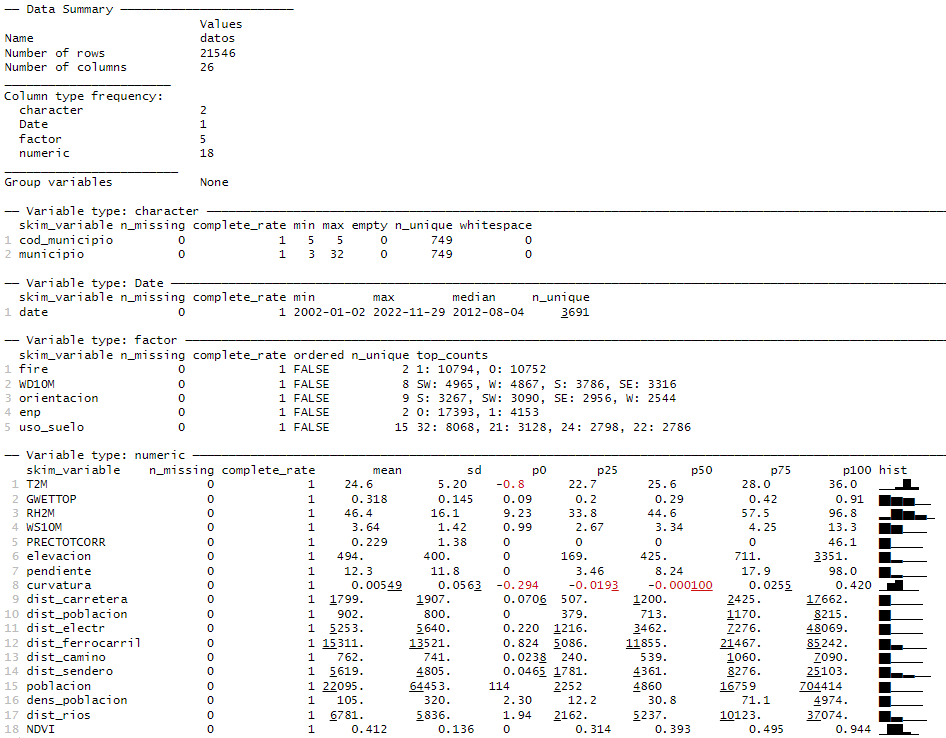
\includegraphics[width = \textwidth]{graficos/skim_datos.png}
\caption{Incendios durante el periodo de estudio}
\label{fig:skim_datos}
\end{figure}

\hypertarget{distribuciuxf3n-de-la-variable-objetivo}{%
\subsection{Distribución de la variable
objetivo}\label{distribuciuxf3n-de-la-variable-objetivo}}

En primer lugar, se estudiará la distribución de la \emph{fire} espacial
y temporalmente.

\begin{figure}[htb]
\centering
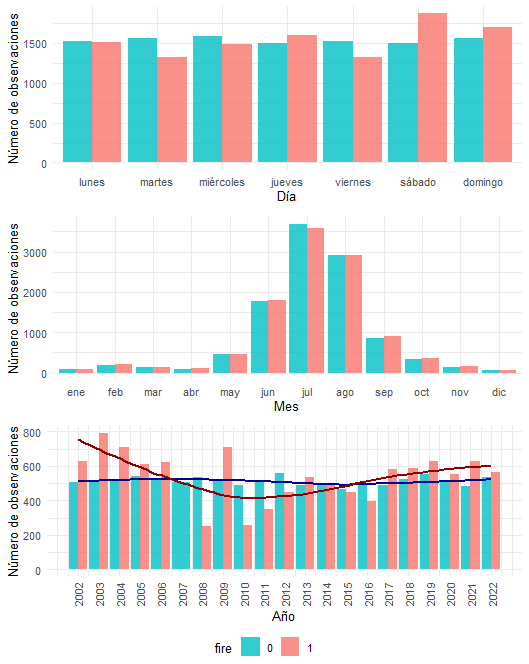
\includegraphics[width = 0.5\textwidth]{graficos/distribucion_temporal_fire.png}
\caption{Distribución temporal de las observaciones en función de la variable objetivo.}
\label{fig:dist_temp_fire}
\end{figure}

En la Figura \ref{fig:dist_temp_fire} se muestran los histogramas de la
variable objetivo en función del día de la semana, del mes y del año,
respectivamente. En primero de ellos se observa que mientras que la
distribución de los casos negativos es uniforme entre los días de la
semana, en los casos positivos se aprecia un ligero aumento en el fin de
semana, especialmente en el sábado. En el segundo histograma, se observa
como las observaciones se concentran en los meses de verano y en cada
mes hay una cantidad balancedada de muestras de ambas clases (esto es
fruto del proceso de muestreo de las observaciones negativas, que como
se ha explicado en la sección anterior, se ha llevado acabo asegurando
que la proporción de casos negativos en cada mes sea igual a la de los
casos positivos). En el tercer histograma es remarcable que, mientra las
observaciones negativas están uniformemente distribuidas entre los 20
años del estudio, las positivas muestran una disminución importante en
los años 2008 y 2010. En el año 2007 no hay observaciones positivas,
debido a que los 4 polígonos de incendios mayores de 100ha que había
registrados ese año no disponían de la fecha de inicio del incendio, por
lo que no pudieron usarse para el estudio. Se desconoce la causa del
reducido número de incendios (mayores de 100ha) en 2007, 2008 y 2010.

Dada la clara influencia el mes y la aparente influencia del día de la
semana en la aparición de incendios, estas variables serán incluidas en
los modelos a través del procesamiento de la variable \emph{date}.

\begin{figure}[h]
\centering
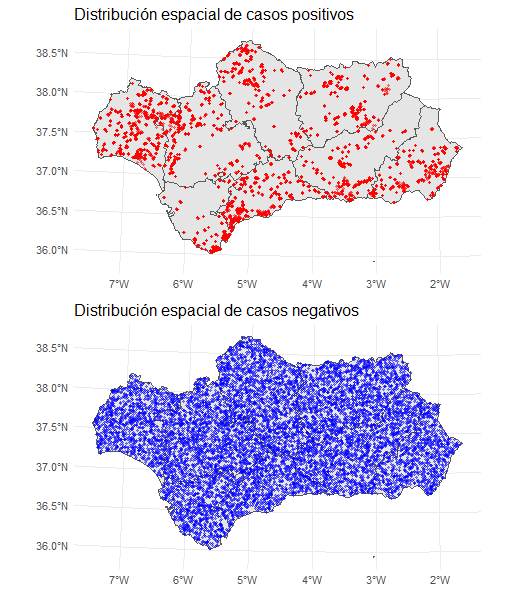
\includegraphics[width = 0.5\textwidth]{graficos/distribucion_espacial_fire.png}
\caption{Distribución espacial de las observaciones en función de la variable objetivo.}
\label{fig:dist_spat_fire}
\end{figure}

En la Figura \ref{fig:dist_spat_fire} se observa claramente como las
\(10752\) muestras negativas están uniformemente distribuidas dentro de
los límites de la Comunidad Autónoma de Andalucía, mientras que las
\(10794\) muestras positivas se concentran a ambos lados de la cuenca
del río Guadalquivir, con una mayor densidad de observaciones en la
provincia de Huelva y en algunas zonas de la costa mediterránea (como ya
se apreciaba en la Figura \ref{fig:area_fuego}).

\hypertarget{anuxe1lisis-univariantes-variables-numuxe9ricas}{%
\subsection{Análisis univariantes variables
numéricas}\label{anuxe1lisis-univariantes-variables-numuxe9ricas}}

El análisis univariante de las variables numéricas se lleva a cabo desde
3 enfoques complementarios:

\begin{enumerate}
\def\labelenumi{\arabic{enumi}.}
\item
  A través de la los resúmenes numéricos recogidos en la Figura
  \ref{fig:skim_datos} y del análisis gráfico de los diagramas de caja y
  bigote (\ref{fig:boxplots}).
\item
  Estudiando la media mensual de cada variable en función de la variable
  \emph{fire}.
\item
  Analizando la distribución espacial de cada variable separando por mes
  si corresponde.
\end{enumerate}

\begin{figure}[]
\centering
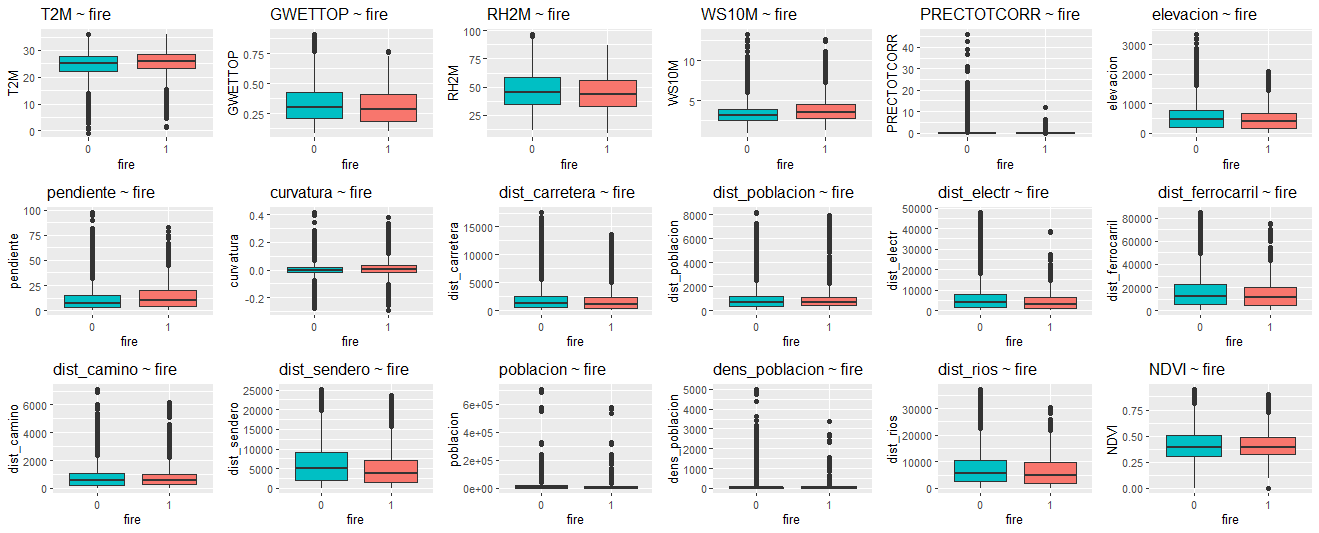
\includegraphics[width =0.5\textwidth]{graficos/boxplots.png}
\caption{Boxplot de cada variable numérica en función de la variable objetivo.}
\label{fig:boxplots}
\end{figure}

En los \emph{boxplots} de las variables numéricas en función de la
variable \emph{fire} (\ref{fig:boxplots}) destacan varios aspectos. Por
un lado, como ya se había comentado anteriormente, que las variables
presentan escalas muy diferentes y que la mayoría de las variables
tienen una marcada asimetría hacia la derecha. Por otro lado, es
evidente la gran cantidad de valores \emph{outliers} que se observan en
los datos, lo que tendrá implicaciones en los modelos que se construyan
con ellos. Sin embargo, es importante destacar que no se trata de
observaciones erróneas, si no que son inhenerentes a la naturaleza de
los datos. Por ejemplo, en el caso de la variable \emph{PRECTOTCORR} el
valor máximo observado es 46.06mm en un día, un valor elevado que sin
duda es atípico en esta región de clima seco, pero sin embargo, posible.
Es también remarcable que todas las variables presentan una variabilidad
similar en ambos niveles del factor \emph{fire}, lo que indica que no
será un problema de clasificación trivial. A priori, solo con los
diagramas de caja y bigotes y los resúmenes numéricos es difícil llegar
sacar más conclusiones, sin embargo, sí pueden observarse sutiles
diferencias entre las distribuciones de algunas variables para ambos
niveles del factor \emph{fire}.

Dada la naturaleza temporal de algunas variables, el análisis gráfico de
los \emph{boxplots} resulta insufiente. Con el fin de considerar la
componente estacional de las variables climáticas y de vegetación, a
continuación, se estudiará la media mensual de cada una de estas
variables función de la variable objetivo.

\begin{figure}[H]
\centering
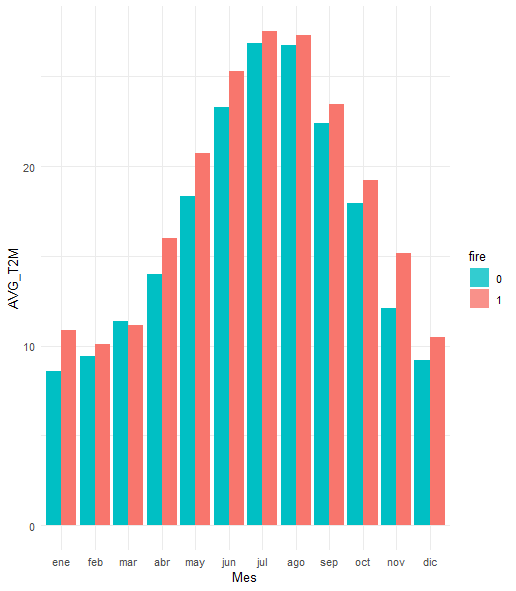
\includegraphics[width = 0.5\textwidth]{graficos/T2M_mes.png}
\caption{Media mensual de la temperatura en función de fire.}
\label{fig:T2M_mes}
\end{figure}

En la Figura \ref{fig:T2M_mes} se puede observar como en casi todos los
meses, la temperatura media mensual es superior en las observaciones en
las que se ha registrado un incendio forestal.

\begin{figure}[H]
\centering
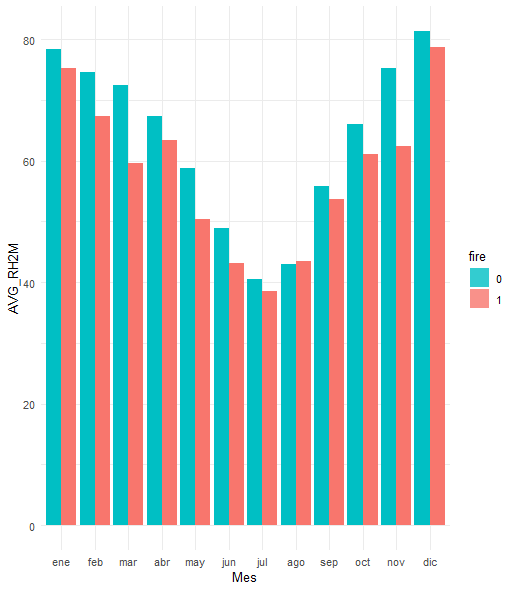
\includegraphics[width =0.5\textwidth]{graficos/RH2M_mes.png}
\caption{Media mensual de la humedad relativa en función de fire.}
\label{fig:RH2M_mes}
\end{figure}

En la Figura \ref{fig:RH2M_mes} se puede observar que en todos los meses
la media mensual de la humedad relativa del aire a 2m sobre la
superficie es menor en las observaciones en las que se ha registrado un
incendio forestal. Sin embargo, las diferencias se reducen durante los
meses de verano, en los que la humedad presenta valores bajos en ambas
clases.

\begin{figure}[H]
\centering
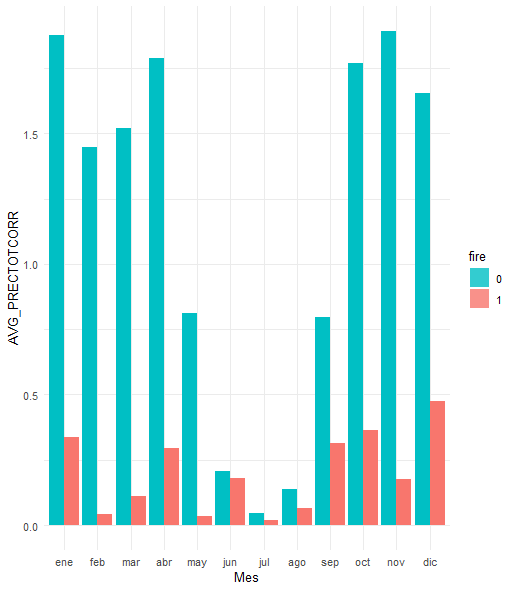
\includegraphics[width =0.5\textwidth]{graficos/PRECTOTCORR_mes.png}
\caption{Media mensual de la precipitaciones en función de fire.}
\label{fig:PRECTOTCORR_mes}
\end{figure}

En la Figura \ref{fig:PRECTOTCORR_mes} se observa una clara diferencia
en la media mensual de las precipitaciones diarias en función del de si
se ha registrado o no un incendio forestal en la observación, siendo
significativamente mayor en este último caso.

\begin{figure}[H]
\centering
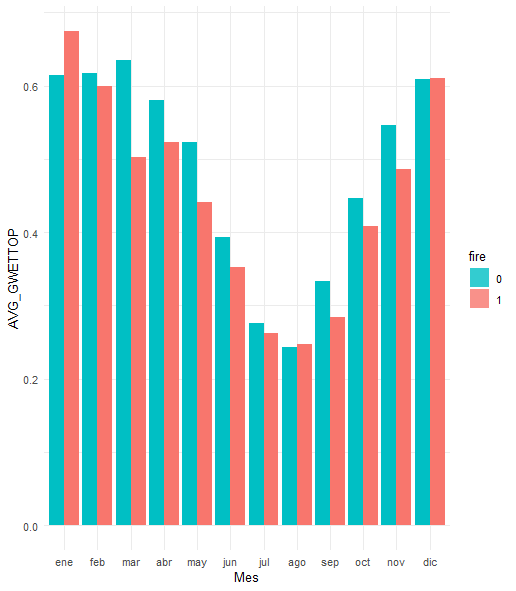
\includegraphics[width =0.5\textwidth]{graficos/GWETTOP_mes.png}
\caption{Media mensual de la humedad del suelo en función de fire.}
\label{fig:GWETTOP_mes}
\end{figure}

En la Figura \ref{fig:GWETTOP_mes} se observa un gráfico similar al de
la humedad relativa del aire, con valores medios más elevados en las
observaciones en las que no se han registrado incendio forestal. Sin
embargo, también parece que las diferencias son más reducidas durante la
estación estival.

\begin{figure}[H]
\centering
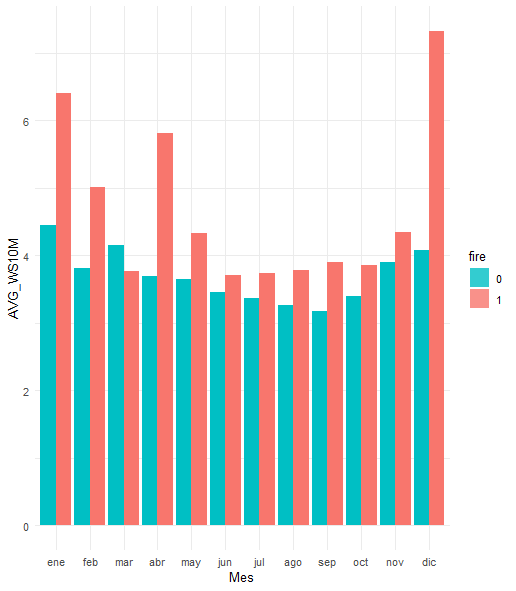
\includegraphics[width = 0.5\textwidth]{graficos/WS10M_mes.png}
\caption{Media mensual de la humedad del suelo en función de fire.}
\label{fig:WS10M_mes}
\end{figure}

En la Figura \ref{fig:WS10M_mes} se observa como durante todos los
meses, la media mensual de la velocidad del viento a 10 metros sobre la
superficie es mayor en los registros en los que ha habido un incendio
forestal.

\begin{figure}[H]
\centering
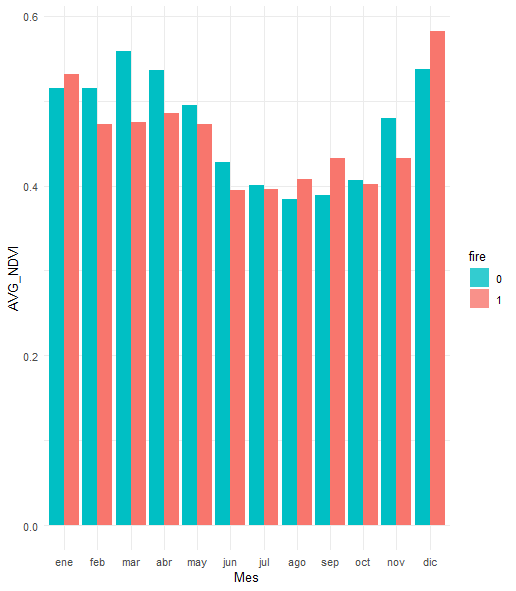
\includegraphics[width = 0.5\textwidth]{graficos/NDVI_mes.png}
\caption{Media mensual de la humedad del suelo en función de fire.}
\label{fig:NDVI_mes}
\end{figure}

Como se observa en la Figura \ref{fig:NDVI_mes}, las diferencias entre
los casos en los que se ha registrado incendio y los que no en términos
del \emph{NDVI} no están claras.

En el {[}Apéndice: Gráficos espaciales EDA{]} se recogen los gráficos
espaciales y espacio\_temporales de todas las variables numéricas. En
ellos se refleja como la valores de las variables en estudio son
coherentes con lo que cabría esperar de la realidad. Además, permiten
una comprensión mayor de la distribución espacial (y temporal) de las
variables en el área de estudio, lo que será útil de cara a interpretar
los modelos que se construyan.

\hypertarget{anuxe1lisis-multivariantes-de-las-variables-numuxe9ricas}{%
\subsection{Análisis multivariantes de las variables
numéricas}\label{anuxe1lisis-multivariantes-de-las-variables-numuxe9ricas}}

En la Figura \ref{fig:corrplot} se muestra un gráfico con las
correlaciones entre las variables. La interpretación es sencilla, cuanto
más intenso sea el color y cuanto mayor sea la excentricidad de la
elipse, mayor será la correlación (en valor absoluto) para ese par de
variables. El color de la elipse indica el signo del coeficiente de
correlación. De esta forma, se observa que las variables más
correlacionadas en la muestra son:

\begin{itemize}
\tightlist
\item
  \emph{T2M} con \emph{RH2M} (negativamente, -0.71)
\item
  \emph{T2M} con \emph{GWETTOP} (negativamente, -0.69)\\
\item
  \emph{GWETTOP} con \emph{R2HM} (positivamente, 0.68)
\item
  \emph{poblacion} con \emph{dens\_poblacion} (positivamente,0.63)
\end{itemize}

\begin{figure}[h]
\centering
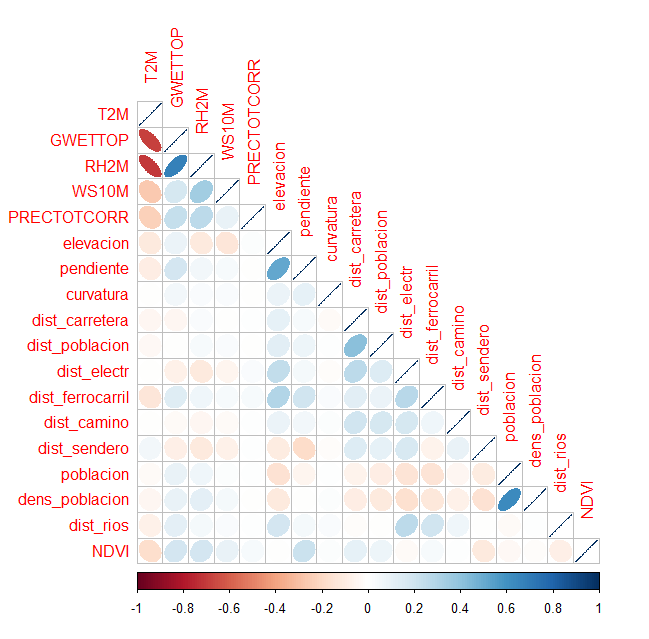
\includegraphics[width =\textwidth]{graficos/corrplot.png}
\caption{Correlaciones entre variables numéricas}
\label{fig:corrplot}
\end{figure}

En la Figura \ref{fig:parcoord} se muestra el gráfico de coordenadas
paralelas de las variables tipificadas a una normal estándar, es decir,
restándoles la media y dividiendo por la desviación típica. Este gráfico
complementa la información de los \emph{boxplots}, pues refleja también
las relaciones entre las variables. Si bien es cierto que al tener un
número bastante elevado de observaciones el gráfico no es tan claro,
pueden hacerse algunas observaciones importantes.

En primer lugar, se observa que la variable con mayor variabilidad (una
vez tipificada) es PRECTOTCORR, que presenta bastantes valores atípicos,
todos ellos en observaciones en las que no se ha registrado incendio.
También destacan en este sentido \emph{dens\_poblacion} y
\emph{poblacion}, entre las que además puede observarse que no hay una
relación lineal clara (hay municipios con un elevado número de
habitantes pero con una densidad de población reducida y viceversa).
Además, puede verse que todas las variables tienen una marcada asimetría
positiva (salvo \emph{curvatura}, \emph{T2M} y \emph{NDVI}). Este
gráfico es útil también pues permite ver a que clase de \emph{fire}
corresponden los valores más atípicos de cada variable. Por ejemplo: la
mayor parte de los valores más elevados de \emph{WS10M},
\emph{dist\_poblacion}, \emph{curvatura} y \emph{dist\_camino} se dan en
observaciones positivas, mientras que en \emph{PRECTOTCORR},
\emph{elevacion}, \emph{GWTTOP}, \emph{dist\_Carretera},
\emph{dist\_electr} y \emph{dist\_rios} sucede lo contrario.

\begin{figure}[h]
\centering
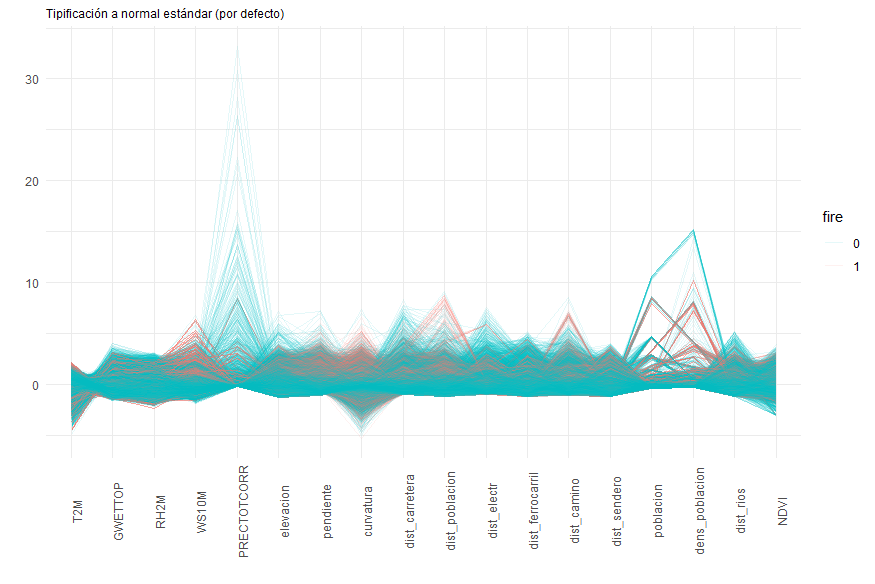
\includegraphics[width =\textwidth]{graficos/parcoord.png}
\caption{Gráfico de coordenadas paralelas.}
\label{fig:parcoord}
\end{figure}

Los resultados de aplicar análisis de componentes principales sobre la
matriz de correlaciones de las 18 variables numéricas se muestran en la
Figura \ref{fig:PCA}. Como se puede observar, se necesitan al menos 11
componentes principales para lograr explicar el 80\% de la varianza de
la muestra, y 14 para alcanzar el 90\% de la varianza de los datos.
Estos resultados se aplicarán más adelante en los modelos, pero a nivel
meramente explicativo ya indican que se trata de un conjunto de datos
complejo en cuanto a la dimensión real de estos.

\begin{figure}[h]
\centering
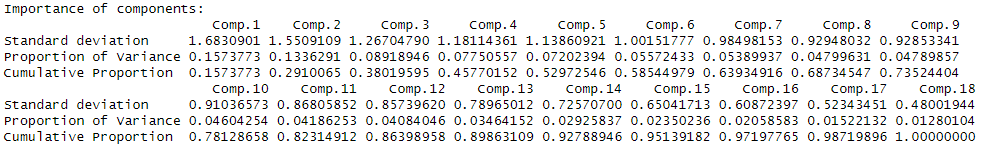
\includegraphics[width =\textwidth]{graficos/pca.png}
\caption{PCA sobre la matriz de correlaciones de las variables numéricas}
\label{fig:PCA}
\end{figure}

\hypertarget{anuxe1lisis-de-las-variables-categuxf3ricas}{%
\subsection{Análisis de las variables
categóricas}\label{anuxe1lisis-de-las-variables-categuxf3ricas}}

Las variables categóricas se analizarán a través de los histogramas de
cada variable en función de la variable \emph{fire} (Figura
\ref{fig:histogramas}).

En la variable \emph{WD10M} cabe destacar la escasez de observaciones
con dirección del viento norte. En el histograma no se observa una clara
relación de esta variable con la variable objetivo, aunque entre las
observaciones con viento con dirección sur o suroeste hay más
observaciones negativas y entre las que tienen dirección noroeste o este
hay una mayor presencia de observaciones positivas.

En el caso de la variable \emph{orientación}, la relación tampoco está
clara, aunque puede verse una mayor proporción de observaciones
positivas en las superficies con orientación sur (sureste, sur y
suroeste).

En términos de la variable \emph{enp} por si sola no se observan
diferencias significativas entre ambas clases.

La variable \emph{uso\_suelo} sí que muestra una distribución
marcadamente diferenciada entre ambas clases. La mayoría de las
observaciones positivas se dan en espacios de vegetación arbustiva y/o
herbácea, clase en la que hay casi el doble de observaciones positivas
que negativas. En tierras de labor y cultivos permanentes la proporción
de observaciones negativas es mucho mayor, mientras que en zonas
agrícolas heterogéneas y en espacios abiertos con poca o sin vegetación
hay una mayor presencia de observaciones positivas. También es relevante
el hecho de que casi la totalidad de las observaciones se encuentran en
zonas agrícolas y en zonas forestales, mientras que en las demás clases
la proporción de observaciones es mucho menor (\(3.5%
\) de total). Es por ello que antes de construir los modelos, todas las
categorías categorías de uso de suelo que no se corresponden con zonas
agrícolas o forestales (es decir, todas cuyo código no comience por 2 o
3) se agruparán en el nivel \emph{Otro}. En \ref{fig:uso_suelo} puede
observarse la distribución espacial de esta variable.

\begin{figure}[h]
\centering
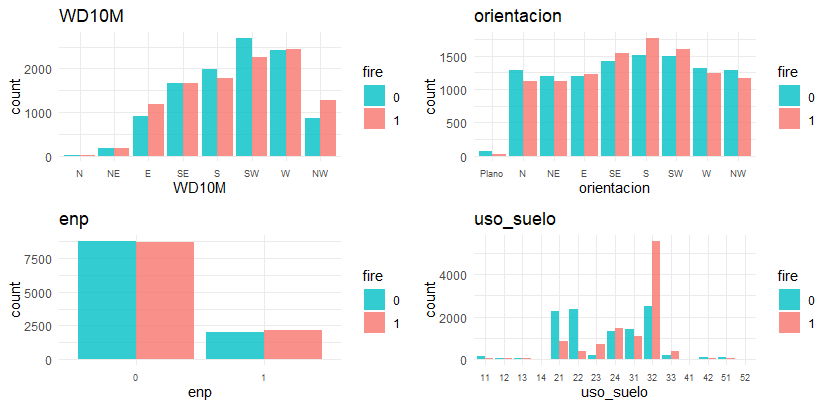
\includegraphics[width =\textwidth]{graficos/histogramas.png}
\caption{Histogramas de las variables categóricas en función de fire.}
\label{fig:histogramas}
\end{figure}

\hypertarget{modelizaciuxf3n}{%
\section{Modelización}\label{modelizaciuxf3n}}

A continuación se va a utilizar el conjunto de datos construido en el
capítulo {[}Construcción del conjunto de datos{]} para entrenar los
modelos de clasificación binaria explicados en la sección {[}Modelos{]}.
Es evidente que el rendimiento de los modelos debe evaluarse en
observaciones futuras, por lo que las técnicas habituales de validación
cruzada o partición aleatoria en entrenamiento/test no son adecuadas
para este problema, ya que sufrirían el llamado efecto
\emph{look-ahead}. Por tanto, el enfoque que se seguirá en este trabajo
será trabajar con una partición en entrenamiento/validación/test
construida a partir de la ordenación temporal de las observaciones.

Se compararán los resultados obtenidos en 7 modelos diferentes:
Regresión logística con penalización, Regresión logística con
penalización + PCA, Árboles de decisión,Bosques aleatorios, KNN, SVM
lineal y SVM radial.

Se ha seguido el flujo de trabajo habitual de \emph{tidymodels}:

1º. Crear una partición temporal en entrenamiento (60\%), validación
(20\%) y test (20\%), que será utilizada en todos los modelos.

2º. Definir cada uno de los modelos, indicando los parámetros del modelo
deberán ajustarse.

3º. Crear la receta (\emph{recipe}) con el preprocesamiento que se usará
en cada modelo. Como se observó en la sección
\protect\hyperlink{anuxe1lisis-exploratorio-de-datos}{Análisis
exploratorio de datos}, se incluirán en todos los modelos variables
categóricas que indiquen el día de la semana y el mes de cada
observación, haciendo uso de la función \texttt{step\_date}. Igualmente,
como también se indicó en el EDA, se modificará la variable
\emph{uso\_suelo} para unificar todos los niveles que no sean agrícolas
o forestales en un solo nivel que se llamará \emph{Otro}. Esto último se
hará fuera del \emph{workflow}, antes de realizar la partición del
conjunto de datos, haciendo uso de la función \texttt{fct\_lump} del
paquete \emph{forcats}. Los detalles del preprocesamiento que se ha
llevado a cabo en cada modelo pueden consultarse en el código, que se
adjunta en el Apéndice 2, donde aparecen debidamente comentados. 4º.
Crear el \emph{workflow} con el modelo y la receta.

5º. Crear la rejilla (\emph{grid}) con los posibles valores de los
parámetros que se deben ajustar.

6º. Entrenar el modelo para cada combinación de los valores de los
parámetros a ajustar sobre los datos de entrenamiento.

7º. Evaluar el rendimiento de cada modelo sobre los datos de validación
y seleccionar el mejor en base a las medidas de rendimiento ya
mencionadas. El objetivo con estos modelos es predecir incendios
forestales, por lo que es de vital importancia que los modelos funcionen
especialmente bien en la clase positiva, es decir, que si un incendio se
va a producir, que el modelo lo detecte. Sin embargo, es fundamental que
el modelo tenga un buen desempeño general (un modelo que todo lo
clasifique como incendio no serviría de nada, poniendo un ejemplo
extremo). Por tanto, cada modelo se valorará de forma individual,
considerando todas las métricas de rendimiento mencionadas y priorizando
la sensitividad (o \emph{recall}). Sin embargo, en la mayoría de los
casos maximizar la tasa de acierto maximiza también la sensitividad,
garantizando además un buen desempeño general. Por ello, en la mayoría
de modelos se maximizará la tasa de acierto, pero porque analizando las
salidas individualmente se ha considerado que es la mejor opción ya que
produce la mayor sensitividad sin bajar demasiado las otras medias.

\hypertarget{regresiuxf3n-loguxedstica-con-penalizaciuxf3n}{%
\subsection{Regresión logística con
penalización}\label{regresiuxf3n-loguxedstica-con-penalizaciuxf3n}}

Antes de aplicar este modelo, se han transformado las variables
categóricas a variables \emph{dummy} y se han tipificado todas las
variables (media 0 y varianza 1).Los parámetros a ajustar son
\(\lambda\) (parámetro de penalización o \emph{penalty}) y \(\alpha\)
(parámetro de mixtura o \emph{mixture}). Se consideran 10 valores
equiespaciados para cada parámetro (en el caso de \(\lambda\) entre
\(10^{-4}\) y \(10^{-1}\) y el caso de \(\alpha\) entre \(0\) y \(1\)) y
se construye el grid tomando todas las combinaciones de estos valores.

Las métricas obtenidas por cada combinación de parámetro sobre los datos
de validación se representan en la Figura \ref{fig:lr_tuningplot}

\begin{figure}[h!]
\centering
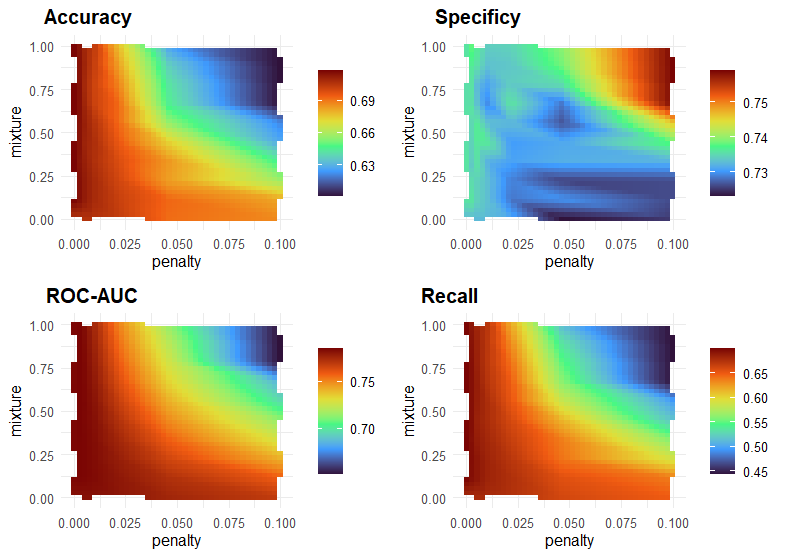
\includegraphics[width =0.7\textwidth]{graficos/lr_tuningplot.png}
\caption{Métricas de rendimiento de los modelos de regresión logística con penalización.}
\label{fig:lr_tuningplot}
\end{figure}

Finalmente, se elige el modelo maximiza la tasa de acierto, cuyos
parámetros son: \(\alpha= 1\) y \(\lambda = 0.000464\). Es decir, un
modelo de regresión logística \emph{lasso} puro. Los coeficientes de
este modelo se muestran en la Figura \ref{fig:lr_coef}.

\hypertarget{regresiuxf3n-loguxedstica-con-penalizaciuxf3n-pca}{%
\subsection{Regresión logística con penalización +
PCA}\label{regresiuxf3n-loguxedstica-con-penalizaciuxf3n-pca}}

A continuación se considera el mismo modelo de regresión logística con
penalización que en la sección anterior pero en lugar de trabajar con
los datos directamente, se aplica análisis de componentes principales
sobre los datos normalizados en el preprocesamiento, ajustando el número
de componentes principales utilizadas. Para construir el \emph{grid} de
parámetros se consideran los mismos valores que en el modelo sin PCA
para los parámetros de penalización y mixtura pero ahora se consideran
también 7 posibles valores para el número de componentes principales
(\(\{20,25,30,...,50\}\)). Finalmente, el modelo que maximiza la tasa de
acierto es el que tiene 40 componentes principales, \(\alpha= 0.333\) y
\(\lambda = 0.00464\).

\hypertarget{uxe1rboles-de-decisiuxf3n}{%
\subsection{Árboles de decisión}\label{uxe1rboles-de-decisiuxf3n}}

Se construirán los árboles de decisón usando el índice de Gini como
función de impureza y se elegirá el parámetro de coste-complejidad
(\(\alpha\)) que maximice la tasa de acierto. Se considera un
\emph{grid} con 10 valores del parámetro de coste-complejidad que
oscilan entre \(1.28e-10\) y \(3.02e- 2\). La mejor tasa de acierto en
el conjunto de validación se obtiene con \(\alpha = 0.00182\). En la
Figura \ref{fig:dt_tuningplot} se muestran las distintas métricas de
rendimiento sobre los datos de validación para cada uno de los valores
del parámetro a ajustar.

\begin{figure}[h!]
\centering
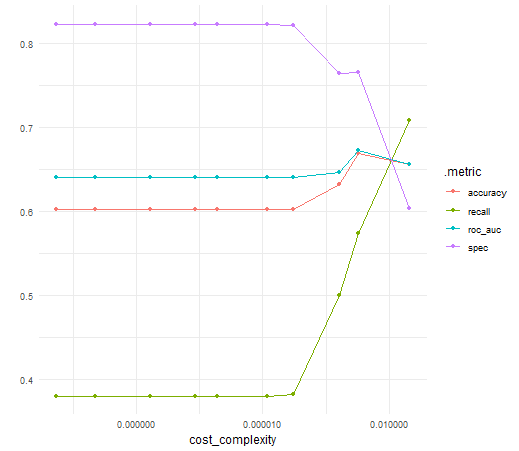
\includegraphics[width =0.7\textwidth]{graficos/dt_tuningplot.png}
\caption{Métricas de rendimiento del árbol de decisión en función de el parámetro de coste\-complejidad.}
\label{fig:dt_tuningplot}
\end{figure}

\hypertarget{bosques-aleatorios}{%
\subsection{Bosques aleatorios}\label{bosques-aleatorios}}

En este modelo se ha fijado el número de árboles a 1000 y se han
ajustado los parámetros \emph{mtry} (el número de variables que se
seleccionarán aleatoriamente en cada nodo) y \emph{min\_n} (el número de
observaciones en un nodo a partir del cual no se sigue dividiendo y se
convierte en nodo hoja). En este caso se ha optado por un enfoque
diferente, motivado por el amplio rango de valores que puede tomar el
parámetro \emph{min\_n} y por las limitaciones computacionales del
equipo disponible.

De esta forma, la estimación de parámetros se ha hecho en dos etapas. En
una primera etapa se ha fijado el parámetro \(mtry = 4\) y se ha
estimado el parámetro \emph{min\_n} considerando para ello un
\emph{grid} equiespaciado de 1000 a 2500 tomando valores de 100 en 100
(\(\{1000,1100,...,2500\}\)). Para elegir entre los distintos modelos
esta vez se ha usado como criterio la sensitividad, obteniendo el valor
más elevado para \(min\_n = 2100\). En la segunda etapa, una vez
\emph{min\_n}, este se ha considerado fijo y se ha estimado
\emph{m\_try}, considerando una rejilla de 10 valores equiespaciados
tomados del 1 al 10 (\(\{1,2,...,10\}\)). De nuevo se ha utilizado la
sensitividad para elegir el modelo final, eligiendo así \(min\_n = 7\).
En la Figura \ref{rf_tuningplot} se recogen los resultados de las dos
estapas de \emph{tuning}. El modelo final elegido tiene
\(min\_n = 2100\) y \(min\_n = 7\).

\begin{figure}[h!]
\centering
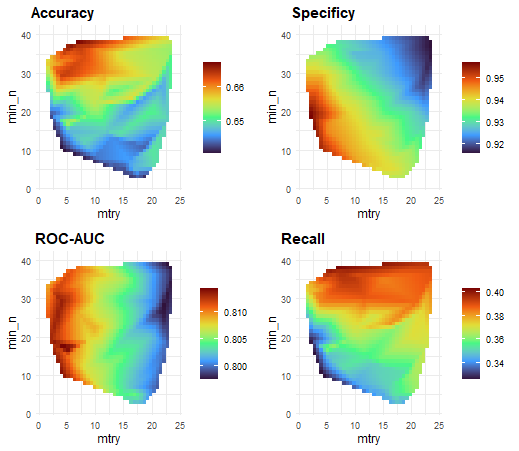
\includegraphics[width =0.7\textwidth]{graficos/rf_tuningplot.png}
\caption{Métricas de rendimiento de Random Forest en función de los parámetros.}
\label{fig:rf_tuningplot}
\end{figure}

\hypertarget{knn}{%
\subsection{KNN}\label{knn}}

Para aplicar el modelo, primero se han transformado las variables
categóricas en variables \emph{dummy} y, porsteriormente, se han
tipificado las todas las variables. Se ha usado la distancia euclídea
entre los vectores transformados. Para ajustar el parámetro \(k\) del
modelo se han tomado valores entre 1 y 400. La mayor tasa de acierto
sobre los datos de validación se ha obtenido con \(k = 275\). Los
resultados del \emph{tuning} se muestran en la Figura
\ref{fig:knn_tuningplot}.

\begin{figure}[h!]
\centering
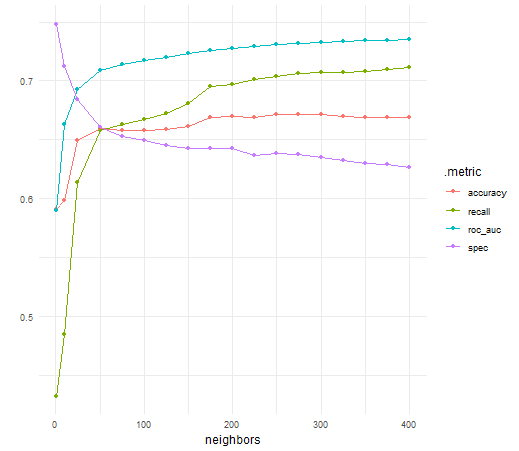
\includegraphics[width =0.7\textwidth]{graficos/knn_tuningplot.png}
\caption{Métricas de rendimiento de KNN en función del número de vecinos.}
\label{fig:knn_tuningplot}
\end{figure}

\hypertarget{svm-lineal}{%
\subsection{SVM lineal}\label{svm-lineal}}

Antes de construir el modelo, se han transformado las variables
categóricas usando variables \emph{dummy} y se han tipificado todas las
variables. Se ha probado con 15 valores del parámetro \emph{coste} entre
0.001949 y 24.666648. La mayor tasa de acierto y el mayor \emph{recall}
se han obtenido para \(C = 0.0437\). Los resultados del \emph{tuning} se
muestran en la Figura \ref{fig:svm_tuningplot}

\begin{figure}[h!]
\centering
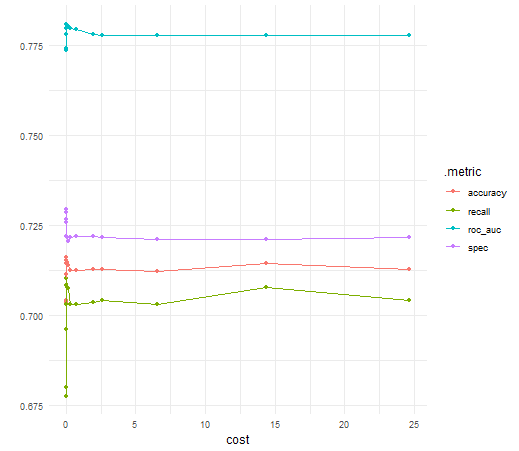
\includegraphics[width =0.7\textwidth]{graficos/svm_tuningplot.png}
\caption{Métricas de rendimiento de svm en función del coste.}
\label{fig:svm_tuningplot}
\end{figure}

\hypertarget{svm-radial}{%
\subsection{SVM radial}\label{svm-radial}}

Por último, se ha construido el modelo de SVM usando un kernel
gaussiano. El preprocesamiento ha sido el mismo que en el caso del
kernel lineal. Dado el elevado tiempo de entrenamiento de este modelo
solo se ha probado con 8 combinaciones de valores para los parámetros
\(C\) y \(\gamma\), que oscilan entre 0.005 y 31.7 y entre 0 y 0.05. La
mayor tasa de acierto sobre los datos de validación se ha conseguido
para \(C = 31.7\) y \(\gamma = 0.0000496\).

\hypertarget{comparaciuxf3n}{%
\section{Comparación}\label{comparaciuxf3n}}

A continuación se muestran las métricas de cada uno de los modelos
seleccionados en los datos de validación en la Tabla
\ref{tab:metricas_val} y en la Figura \ref{fig:validation_metrics}. Las
curvas ROC de todos los modelos se muestran en la Figura
\ref{fig:roc_validation}.

\begin{table}[]
\centering
\resizebox{0.5\columnwidth}{!}{%
\begin{tabular}{@{}llllll@{}}
\toprule
model\_name & roc\_auc & accuracy & recall & specificity & precision \\ \midrule
lr          & 0.785    & 0.719    & 0.700  & 0.738       & 0.727     \\
lr\_pca     & 0.727    & 0.659    & 0.624  & 0.694       & 0.670     \\
dt          & 0.656    & 0.656    & 0.709  & 0.604       & 0.641     \\
rf          & 0.781    & 0.725    & 0.758  & 0.693       & 0.711     \\
svm\_linear & 0.781    & 0.716    & 0.710  & 0.722       & 0.718     \\
svm\_rbf    & 0.777    & 0.710    & 0.692  & 0.728       & 0.717     \\
knn         & 0.732    & 0.672    & 0.706  & 0.637       & 0.660     \\ \bottomrule
\end{tabular}%
}
\caption{Métricas de los modelos seleccionados sobre el conjunto de validación.}
\label{tab:metricas_val}
\end{table}

\begin{figure}[h]
\centering
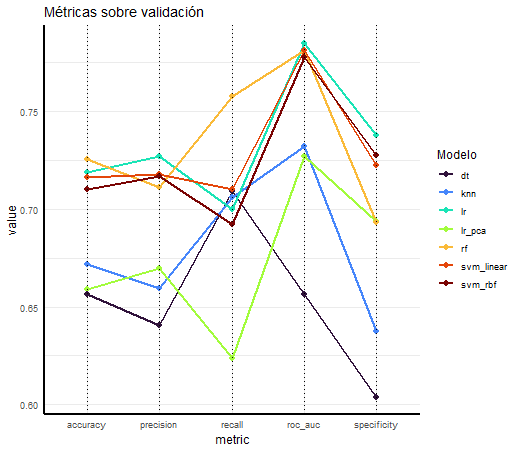
\includegraphics[width =0.7\textwidth]{graficos/validation_metrics.png}
\caption{Métricas obtenidas sobre el conjunto de validación por cada uno de los modelos seleccionados.}
\label{fig:validation_metrics}
\end{figure}

\begin{figure}[h]
\centering
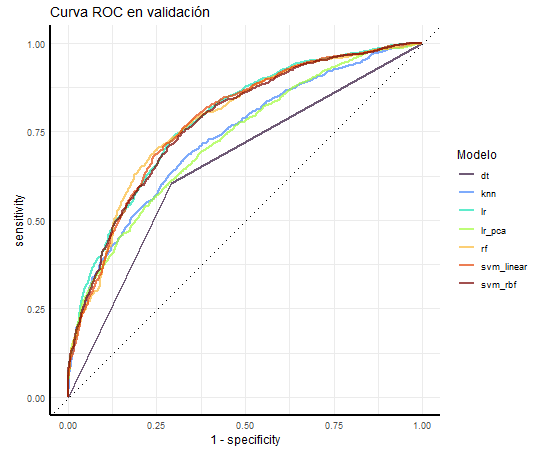
\includegraphics[width =0.7\textwidth]{graficos/roc_validation.png}
\caption{Curvas ROC sobre el conjunto de validación.}
\label{fig:roc_validation}
\end{figure}

Por último, para conocer la capacidad de generalización de los modelos
construidos, estos se evaluarán sobre nuevas observaciones, el conjunto
de datos test. Recuérdese que el entrenamiento de los modelos se ha
realizado con el conjunto de entrenamiento, formado por 12927
observaciones tomadas entre el 2002 y mediados de 2014 y para ajustar
los parámetros de cada modelo, se han utilizado 4309 observaciones
tomadas entre mediados de 2014 y mediados de 2019. Finalmente, se
evaluará la capacidad de predicción de los modelos sobre 4310 nuevas
observaciones tomadas entre mediados de 2019 y 2022. Para ello, primero
se juntarán los conjuntos de entrenamiento y validación para reentrenar
los modelos con la configuración de parámetros seleccionada en cada
caso, y posterior mente se compararán los valores predichos por los
modelos con los valores reales. Los resultados obtenidos se muestran en
la Tabla \ref{tab:metricas_test} y el la Figura \ref{fig:test_metrics}.
Las curvas ROC de los distintos modelos sobre el conjunto de datos test
se muestra en la Figura \ref{fig:roc_test}.

\begin{table}[]
\centering
\resizebox{0.5\columnwidth}{!}{%
\begin{tabular}{@{}llllll@{}}
\toprule
model\_name & roc\_auc & accuracy & recall & specificity & precision \\ \midrule
lr          & 0.795    & 0.710    & 0.726  & 0.693       & 0.718     \\
lr\_pca     & 0.715    & 0.645    & 0.631  & 0.661       & 0.667     \\
dt          & 0.667    & 0.668    & 0.712  & 0.621       & 0.670     \\
rf          & 0.762    & 0.699    & 0.727  & 0.669       & 0.703     \\
svm\_linear & 0.790    & 0.705    & 0.729  & 0.680       & 0.710     \\
svm\_rbf    & 0.789    & 0.706    & 0.727  & 0.683       & 0.712     \\
knn         & 0.744    & 0.673    & 0.719  & 0.624       & 0.673     \\ \bottomrule
\end{tabular}%
}
\caption{Métricas sobre el conjunto test.}
\label{tab:metricas_test}
\end{table}

\begin{figure}[h]
\centering
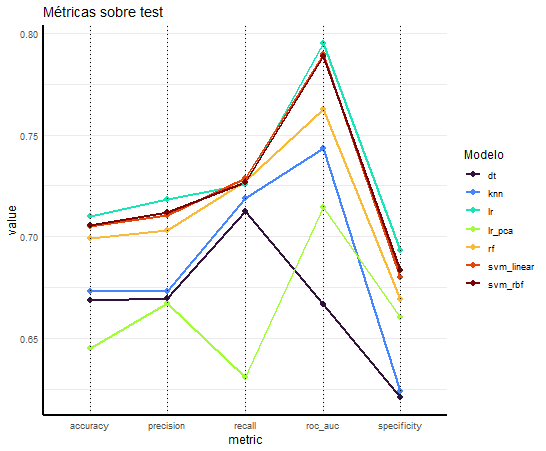
\includegraphics[width =0.7\textwidth]{graficos/test_metrics.png}
\caption{Métricas obtenidas sobre el conjunto test por cada uno de los modelos seleccionados.}
\label{fig:test_metrics}
\end{figure}

\begin{figure}[h]
\centering
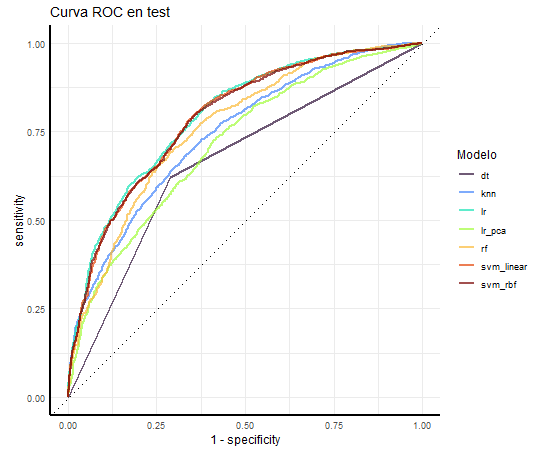
\includegraphics[width =0.7\textwidth]{graficos/roc_test.png}
\caption{Curvas ROC sobre test.}
\label{fig:roc_test}
\end{figure}

\bibliography{bib/library.bib,bib/paquetes.bib}


%


\end{document}
